When working with time series, we often want to determine whether one series causes changes in another. To find this relationship, measuring a cross-correlation and finding a lag is one way how to do it. Lag represents when change in one data series transfers to the other several periods later. 

To ensure a cross-correlation calculation makes sense, first I have to determine, whether are the data stationary. A stationary time series is one whose properties do not depend on the time at which the series is observed\cite{hyndman5forecast}. More precisely, if y\textsubscript{t} is a stationary time series, then for all \textit{s}, the distribution of \textit{(y\textsubscript{t},…,y\textsubscript{t+s})} does not depend on \textit{t}.

To determine whether my data are stationary, I've used the Dickey-Fuller test method of tseries package in R. Results can be seen in the table \ref{table:stationarity_table_sentiment} and \ref{table:stationarity_table_release_count} 

\begin{table}[H]
\centering
\begin{tabular}{ |p{3cm}||p{3cm}|p{3cm}|  }
 \hline
 \multicolumn{3}{|c|}{Stationarity test of web frameworks sentiment data} \\
 \hline
 Framework & Dickey-Fuller & p-value\\
 \hline
 NodeJS   & -2.6775    &0.2964\\ \hline
 AngularJS &   -3.883  & 0.0199\\ \hline
 EmberJS & -4.0783 & 0.0199\\ \hline
 VueJS    &-3.438 & 0.0646\\ \hline
 CakePHP&   -3.480  & 0.04847\\ \hline
 Laravel& -2.57  & 0.3431\\ \hline
 Symfony& -4.3979  & 0.01\\ \hline
\end{tabular}
\caption{Stationarity test of sentiment}
\label{table:stationarity_table_sentiment}
\end{table}

\begin{table}[H]
\centering
\begin{tabular}{ |p{3cm}||p{3cm}|p{3cm}|  }
 \hline
 \multicolumn{3}{|c|}{Stationarity test of web frameworks release count} \\
 \hline
 Framework & Dickey-Fuller & p-value\\
 \hline
 NodeJS   & -2.896    &0.205\\ \hline
 AngularJS &   -2.547  & 0.353\\ \hline
 EmberJS & -3.297 & 0.0802\\ \hline
 VueJS    &-2.158 & 0.511\\ \hline
 CakePHP&   -3.224  & 0.08915\\ \hline
 Laravel& -2.368  & 0.425\\ \hline
 Symfony& -2.218  & 0.488\\ \hline
\end{tabular}
\caption{Stationarity test of release counts}
\label{table:stationarity_table_release_count}
\end{table}

As we can see, p-values are always higher than 0.05 what indicates non-stationarity of the data, therefore I can't calculate the cross-correlation on them in this state. To transform non-stationary data into stationary, 2 approaches can be used. These are differencing and transforming.  I've taken data series and differenced the values in listing \ref{lst:differencing}. I've executed both, seasonal differencing and stationary differencing although seasonal probably was not needed because the data should not be dependant on the season.

\begin{lstlisting}[caption={Used differencing method in R},label={lst:differencing},language=R]
Differencing <- function(x,y)
{
 framework_x_seasdiff <- diff(x,differences=1)  # seasonal differencing
 framework_x_Stationary <- diff(framework_x_seasdiff, differences= 1)
 framework_y_seasdiff <- diff(y, differences=1)
 framework_y_Stationary <- diff(framework_y_seasdiff, differences= 1)
 return(list(framework_x_Stationary,framework_y_Stationary))
}
\end{lstlisting}
New differenced values do appear to be stationary in mean and variance, as the level and the variance of the series stays roughly constant over time. Sentiment for NodeJS before and after differencing can be seen in Figure \ref{fig:NodeJS_Sentiment_before_after}

\begin{figure}[H]%
    \centering
    \subfloat[Before differencing]{{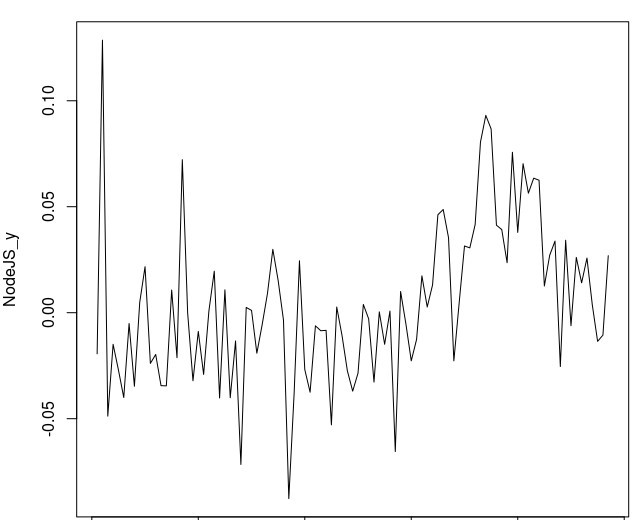
\includegraphics[width=6cm]{NodeJS_before.jpg} }}%
    \qquad
    \subfloat[After differencing]{{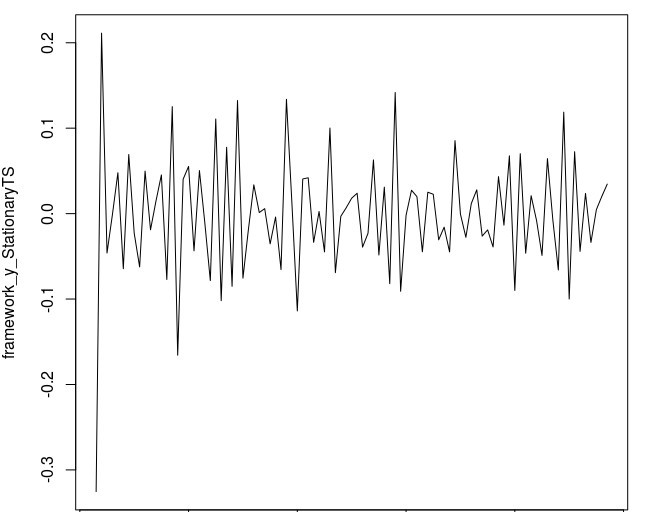
\includegraphics[width=6cm]{NodeJS_after.jpg} }}%
    \caption{NodeJS monthly sentiment values}%
    \label{fig:NodeJS_Sentiment_before_after}%
\end{figure}

Same procedure needed to be done with the "number of releases per month" data and afterwards. Then, cross-correlation could be executed. For this task I've used ccf method in R which implements Pearson's correlation calculation method. Results for all 7 OSS projects can be seen in Figure \ref{fig:highestCorrelationsPlotReleases}

\begin{figure}[H]%
    \centering
	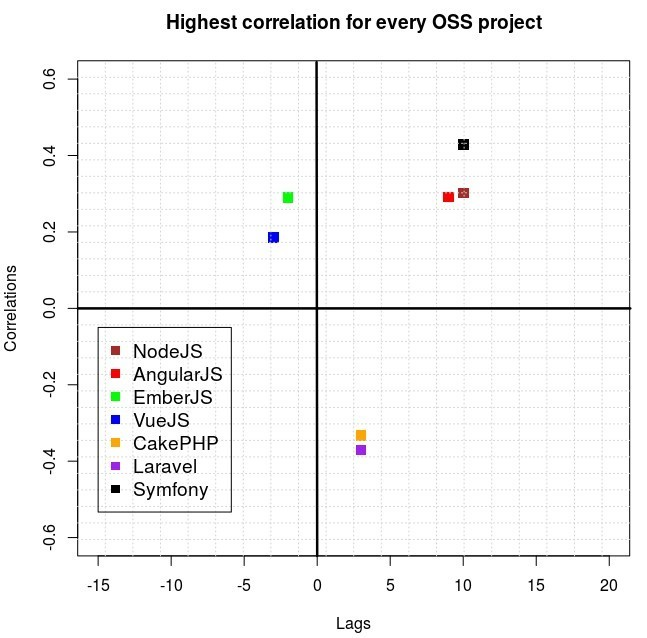
\includegraphics[width=8cm]{highestCorrelationsPlotReleases.jpg}
    \caption{Highest correlations for every OSS project}%
    \label{fig:highestCorrelationsPlotReleases}%
\end{figure}

\paragraph{Results interpretation:}

As we can there is no general pattern. Maximal project correlations happen to occupy 3 of 4 possible quadrants. Each quadrant represents a different relationship between number of releases and sentiment change.

\begin{itemize}
  \item \textbf{I. Quadrant}(Positive correlation + positive lag) - Increase of release count increases a sentiment
  \item \textbf{II. Quadrant}(Positive correlation + negative lag) - Increase of sentiment increases a release count
  \item \textbf{III. Quadrant}(Negative correlation + positive lag) - Increase of release count decreases a sentiment
  \item \textbf{IV. Quadrant}(Negative correlation + Negative lag) - Increase of sentiment decreases a release count
\end{itemize}

Also, in Figure \ref{fig:highestCorrelationsPlotReleases_nonStat} are the results without making the data series stationary. It's obvious that making the data stationary has a big impact on the results.

\begin{figure}[H]%
    \centering
	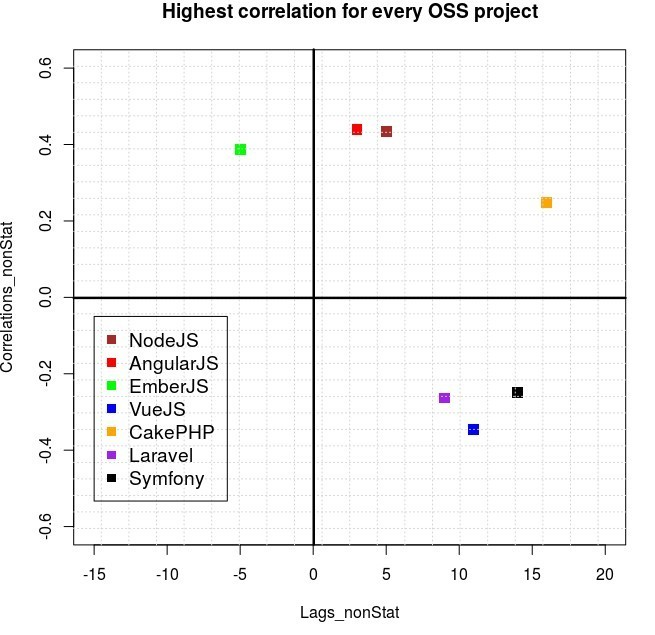
\includegraphics[width=8cm]{highestCorrelationsPlotReleases_nonStat.jpg}
    \caption{Highest correlations for every OSS project (non-stationary)}%
    \label{fig:highestCorrelationsPlotReleases_nonStat}%
\end{figure}